

\documentclass[a4paper,12pt]{book}

\usepackage[spanish]{babel}
\usepackage{graphicx}




\begin{document}


	
	\begin{titlepage}
		\begin{center}
			\vspace*{-1in}
			Universidad de La Habana \\
			Facultad de Matemática y Computación \\
			Departamento de Programación \\
			\vspace*{0.15in}
			\begin{figure}[htb]
				\begin{center}
					
\includegraphics[width=3cm]{./Graphics/uhlogo.pdf}
				\end{center}
			\end{figure}
			
			\vspace*{0.3in}
			\textbf{Título} \\
			\begin{large}
			Generación automática de casos de prueba con aprendizaje de la medida de calidad \\
			\end{large}
			\vspace*{0.6in}
			Autor: \textbf{Marcel Ernesto Sánchez Aguilar} \\
			Tutor: \textbf{Ludwig Leonard Méndez}
			
			
			\vspace*{0.6in}
			Trabajo de Diploma de presentado en opción al título de Licenciado en Ciencia de la Computación
		\end{center}
	\end{titlepage}
	
	

\chapter*{Glosario}
	\begin{itemize}
		\item Software: Conjunto de programas y rutinas que permiten a la computadora realizar determinadas tareas.
		\item Casos de prueba: Conjunto de elementos de entrada que se utilizan para evaluar un programa.
		\item Algoritmo: Secuencia ordenada y finita de operaciones que permiten resolver un problema.
	\end{itemize}
	
\chapter{Introducción}

	La Ciencia de la Computación estudia los fundamentos teóricos de los procesos computacionales y su aplicación en la implementación de sistemas computacionales, en correspondencia con el desarrollo vertiginoso de la propia ciencia y las tecnologías computacionales, los cuales dan solución a la informatización que demanda la sociedad contemporánea. El origen de esta ciencia es anterior a la invención del primer computador moderno, pues desde la antigüedad han existido procedimientos y algoritmos para realizar cómputos, solo que estos eran llevados a cabo por personas y no por un ente digital. Gracias a los trabajos de Alan Turing \cite{Turing} -considerado el padre de esta ciencia- y otros investigadores, se abrió el camino a nuevas ramas como la computabilidad y se profundizó en otras como la Inteligencia Artificial.
	
	Hoy en día la computación ayuda al hombre en casi todas las áreas y muchas tareas que antes se hacían de forma manual, son responsabilidad ahora de un equipo de cómputo. Pero, ¿qué tan bueno puede ser un software y cómo expresamos la calidad de los mismos? El presente trabajo se enfoca en dar solución a un subconjunto de esta problemática: evaluar la calidad de una componte de un software. \\
	
	Las componentes de un software son partes de una aplicación, se dividen en componentes para simplificar la complejidad que resulta la confección de un sistema computacional. Esto facilita el mantenimiento, desarrollo y operaciones que permiten a un mismo código ser usado en varios lugares. Específicamente, se abordará la componente lógica, la cual es vital para el correcto funcionamiento de cualquier sistema de cómputo. 
	
	Una vez fijado el objetivo de evaluación, quedaría por designar las métricas a utilizar para dicho fin. ¿Cómo evaluar una componente de un software? ¿En qué base a cuáles términos se mide la calidad en un sistema de cómputo? Se dará respuesta a las anteriores interrogantes haciendo referencia al estado del arte de este problema.
	
	\section{Estado del Arte}
		La calidad podría resultar fácil de explicar. Sin embargo, no lo es ni en su propia definición. Algunos definen la calidad como el nivel de satisfacción del cliente. Otros dicen que se trata de cumplir con los requisitos del cliente. O bien el estado del software libre de defectos. Para ello se introduce una nueva definición: deuda técnica \cite{EAsoftwareevaluation}. Esto no es más que una serie de aspectos que pueden puntuar la calidad de un software. Se han identificado ocho dimensiones de la deuda técnica del producto de software:
		
		\begin{itemize}
			\item Calidad del código fuente
			\item Usabilidad, interfaz de usuario y documentación
			\item Seguridad
			\item Actuación
			\item Lógica de negocios
			\item Calidad de la arquitectura
			\item Calidad de los datos
			\item Uso de código fuente abierto
		\end{itemize}
	
		Cada dimensión se mide según las métricas críticas y los niveles que deben alcanzar. Permite recibir una evaluación integral del producto con recomendaciones concretas. Con este enfoque, los programadores entienden cómo se siente realmente el producto. Ofrece una evaluación cuantitativa completa de la calidad del producto.
		
		La deuda técnica no es solo acerca del código, este enfoque permite ejecutar un análisis profundo, el cual ha demostrado que las deudas técnicas se refieren a la calidad general del producto. Comprobar el código del software o de una de sus componentes no es suficiente para comprender la eficiencia del producto, se debe avanzar más.
		
	\section{Contexto del problema}

		El proceso de evaluación de las implementaciones de los algoritmos de los estudiantes se realiza de forma semiautomática en la Facultad de Matemática y Computación de la Universidad de La Habana. La generación de los casos de prueba a utilizar es manual y puede resultar engorrosa, pues es necesario cubrir la mayor cantidad de aspectos a evaluar sin incidir de más en algún rasgo para no afectar la calificación. Luego de realizada una generación abarcadora de casos de prueba, se debe escoger ese subconjunto que mejor represente la medida de calidad de efectividad de la componente de software evaluada. % ojo con esto
		
		La idea es proveer al sistema de algunas implementaciones para las cuales se conoce de antemano las evaluaciones y luego se debe encontrar el subconjunto de casos de prueba más cerca de la evaluación de referencia. Luego, si dos soluciones obtienen los mismos resultados al usar idénticos casos de prueba, es muy probable que ambas implementaciones deban obtener la misma calificación. Este es un problema de optimización combinatoria que será abordado con métodos de optimización meta-heurísticos.
		
		
	\section{Resultados esperados, importancia y herramientas a utilizar}
	
		El objetivo general de esta tesis es la generación automática de casos de prueba y la selección o ponderación que permita utilizarlos como medida de calidad para la evaluación de algoritmos. El objeto de investigación es de optimización combinatoria abordado por meta-heurísticas \cite{OptimizacionCombinatoria} para ser aplicado en la definición de los casos de pruebas de las evaluaciones de los estudiantes de Programación en la Facultad de Matemática y Computación. Ahora bien, ¿qué algoritmo implementar? ¿Por qué una meta-heurística? ¿Será necesario aplicar un modelo de optimización? ¿Es un problema de Inteligencia Artificial o de Combinatoria? A estas y otras interrogantes se dará respuesta a lo largo de este documento.
		
		Para el diseño lógico de esta herramienta se utilizará la aplicación Visual Studio y el lenguaje de programación C\#. Esta elección se debe a las facilidades que ambos brindan para la confección de una solución a este problema.
	
	% Objetivos, qué es lo que pienso hacer (app web, herramienta), evaluar la propuesta y compararla con otras 
	% La implementación de la propuesta sería una aplicación de escritorio. \\
	
	% Párrafo que diga la estructura del artículo
    % Este artículo se divide en... \\
	
	% Después viene trabajos relacionados (los que tratan los mismos temas que yo y se utiliza para comparar ideas) y estado del arte (análisis de lo que se ha hecho). Cerrar con una breve crítica.  \\
	% Artículos relacionados, estado del arte, ... \\
	
	% Dar una propuesta
	\section{Ejemplo}
	
	Veamos un ejemplo. El algoritmo de Euclides para hallar el máximo común divisor entre dos números.\\
	
	\textbf{Definición 1.} Máximo Común Divisor de dos números enteros: Es el mayor entero que los divide a ambos sin dejar resto. \\
	
	Entrada: entero $A$, entero $B$ 
	
	Método a implementar: Algoritmo de Euclides.
	
	Salida: $MCD(A, b)$ \\
	
	En este ejemplo, nuestra propuesta debería generar un conjunto de entrada lo suficientemente abarcador, que permita evaluar de forma justa el algoritmo. Por ejemplo, la entrada debería contemplar el cero, los números primos, negativos, de Fibonacci, entre otros.

\chapter{Marco Teórico}
	Los problemas de optimización combinatoria que involucran una extensa pero finita, lista de posibles soluciones son muy comunes en la vida diaria. Por mencionar algunos, entre los problemas más destacados se encuentran el diseño de redes de comunicación y la planificación de rutas de vuelo. Debido a la gran envergadura de estos problemas en cuanto a la cantidad de datos, resulta imposible enumerar las posibles soluciones y quedarnos con la mejor, pues es infactible en tiempo tal enumeración; incluso con los poderes de cómputo actuales, pues dicha lista crece de manera exponencial respecto al tamaño del problema.
	
	En los últimos 50 años se han desarrollado varios métodos de búsqueda, los cuales arrojan una solución factible cercana al óptimo del problema sin necesidad de explorar cada alternativa. Esto es lo que se conoce como Optimización Combinatoria. Debido a esto, se han notado avances significativos en problemas que resultan de importancia para ciencia como lo son el viajante y el enrutamiento de vehículos.
	
	Sin embargo, una buena parte de los problemas encontrados son computacionalmente intratables por su naturaleza o porque son lo suficientemente grandes como para impedir el uso de algoritmos exactos. En tales casos, los métodos heurísticos generalmente se emplean para encontrar soluciones buenas, pero no necesariamente óptimas. La efectividad de estos métodos depende de su capacidad para adaptarse a un ambiente particular, evitar el atrapamiento en los óptimos locales y explotar la estructura básica del problema.
	
	Sobre la base de estas nociones, se han desarrollado diversas técnicas de búsqueda basadas en heurísticas, las cuales han mejorado la capacidad de obtener buenas soluciones a los difíciles problemas de optimización combinatoria. Algunos de los principales métodos son: Recocido Simulado, Búsqueda Tabú, Algoritmos Genéticos y GRASP (Procedimientos de Búsqueda Adaptativa Aleatoria Codiciosos).
	
	\section{Metaheurísticas}
	Algunas de las metaheútistcias que pueden dar solución al problema
		\subsection{Greedy Randomized Adaptive Search Procedures}
		GRASP es una técnica de muestreo aleatorio iterativo. Tiene la invariante de que en cada iteración proporciona una solución factible al problema en cuestión. Hay dos fases dentro de cada iteración del algoritmo: la primera construye inteligentemente una solución a través de una función codiciosa aleatoria; la segunda aplica un procedimiento de búsqueda local a la solución construida con la esperanza de encontrar una mejora.
		
		En la Figura \ref{GRASPgeneral} se muestra el esqueleto general del GRASP%: mientras no se cumpla la condición de parada (línea 2), se construye una solución factible (línea 3), se hace una búsqueda local (línea 4) y se actualiza la solución actual (línea 5).
		
		
		\begin{figure}[h]
			\centering
			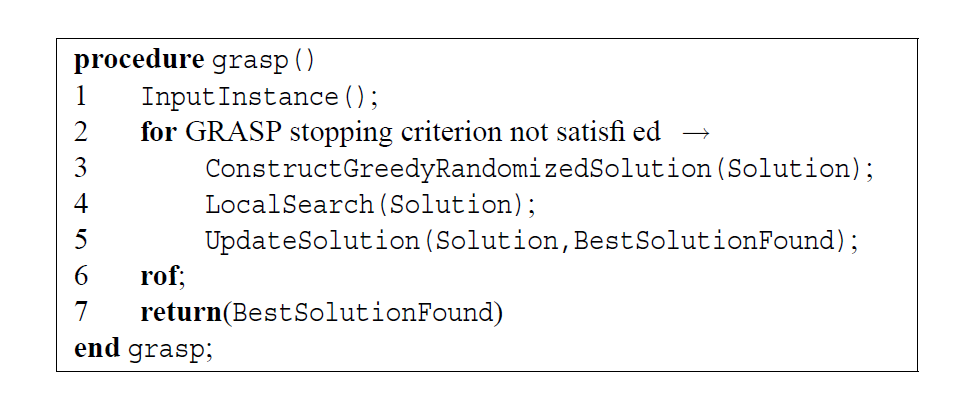
\includegraphics[width=10cm]{./Graphics/GRASPgeneral.png}
			\caption{Algoritmo General GRASP}
			\label{GRASPgeneral}
		\end{figure}
	
		Criterios de parada podrían ser el cumplimiento de un número de iteraciones o el alcance de un valor en la función objetivo. \\
		
		
	
		Ahora se construye iterativamente una solución factible. En cada iteración de construcción, la elección del siguiente elemento a agregar se determina respecto a una función codiciosa. Para reflejar los cambios provocados por la selección del elemento anterior, los beneficios asociados con cada elemento se actualizan en cada iteración. El componente probabilístico de un GRASP se caracteriza por elegir aleatoriamente uno de los candidatos de la lista, pero no necesariamente el mejor candidato. La lista de los candidatos se denomina lista de candidatos restringidos (RCL). Esta técnica de elección permite obtener diferentes soluciones en cada iteración GRASP.
		
		La Figura \ref{GRASPconstructionphase} muestra el pseudocódigo para la fase de construcción de GRASP.
	
		\begin{figure}[h]
			\centering
			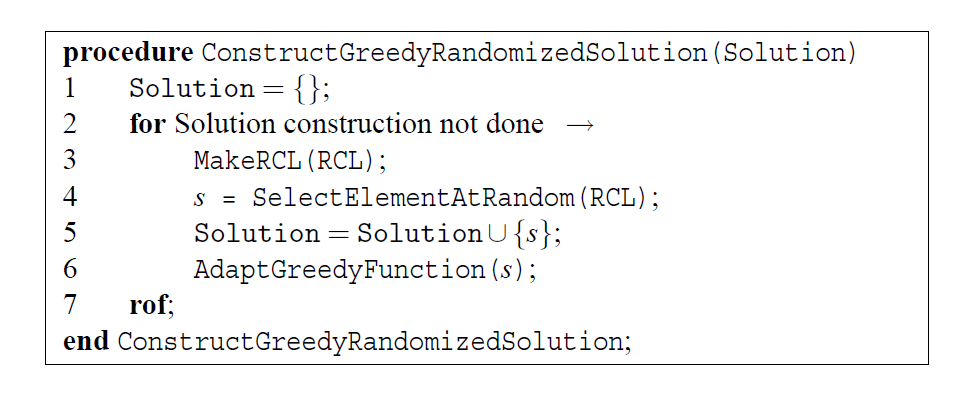
\includegraphics[width=10cm]{./Graphics/GRASPconstructionphase.png}
			\caption{Construcción de la solución GRASP}
			\label{GRASPconstructionphase}
		\end{figure}
	
		El algoritmo de búsqueda local es iterativo y reemplaza sucesivamente la solución actual por una mejor en la vecindad. Termina cuando no se encuentra una solución mejor en el vecindario. La clave del éxito para un algoritmo de búsqueda local consiste en la elección adecuada de una estructura de vecindario, técnicas eficientes de búsqueda y la solución inicial.
		
		A continuación, la Figura \ref{GRASPlocal} muestra dicho procedimiento.
		
		\begin{figure}[h]
			\centering
			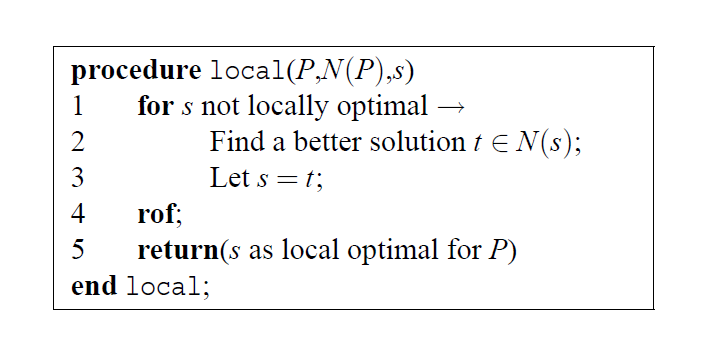
\includegraphics[width=10cm]{./Graphics/GRASPlocal.png}
			\caption{Búsqueda local GRASP}
			\label{GRASPlocal}
		\end{figure}
		
%\begin{thebibliography}{0}
	%\bibitem{id} Fernando Barber y Ricardo Ferrís
%\end{thebibliography}

\bibliography{bibliography}
\bibliographystyle{ieeetr}

\end{document}